\section{Testes}

Nessa seção veremos como o teste está diretamente ligado à qualidade de \textit{software}, os principais tipos de testes, conceitos e ferramentas de automação, veremos quais os tipos de testes que serão aplicados ao nosso projeto e a importância da infra-estrutura de testes em um projeto.


\subsection{Definição}

Segundo o dicionário de termos da IEEE, teste é definido da seguinte forma:

\begin{itemize}
	\item Teste: atividades nas quais um sistema ou um componente é executado sob determinadas condições e os resultados são observados ou gravados, e uma avaliação é feita observando determinado comportamento do sistema ou do componente;
\end{itemize}

\subsection{Teste de Software e Qualidade de Software}

O teste de \textit{software} está diretamente ligado com a qualidade do \textit{software} que está sendo desenvolvido. Podemos ver essa ligação já na definição de qualidade de \textit{software}.

\begin{itemize}
	\item Qualidade de \textit{Software}: Conformidade a requisitos funcionais e de desenvolvimento explicitamente declarados, a padrões de desenvolvimento claramente documentados e a características implícitas que são esperadas de todo \textit{software} profissionalmente desenvolvido.
\end {itemize}

Dentro da qualidade de \textit{software} temos a atividade de garantia de qualidade de \textit{software}, e esta compreende uma variedade de tarefas associadas a sete grandes atividades, entre elas a atividade de testes:

\begin{enumerate}
	\item Aplicação de métodos técnicos;
	\item Realização de revisões técnicas formais;
	\item Atividades de testes de \textit{software};
	\item Aplicação de padrões;
	\item Controle de mudanças;
	\item Medição;
	\item Manutenção de registros e reportagem;
\end{enumerate}

Então podemos estar certos de que se queremos um \textit{software} que atenda aos requisitos especificados, funcionais e não funcionais, que possua uma quantidade de erros reduzida e um desempenho que atenda ao usuário, uma tarefa que não pode ser despensada é o teste da aplicação. Como já dito anteriormente, teste de \textit{software} e qualidade de \textit{software} estão intimamente ligados, na tabela ~\ref{tab:testequalidade} podemos ver quais as características de qualidade são verificadas por determinados tipos de testes.

\begin{table}
	\caption{Tipos de teste e sua característica de qualidade correspondente}
	\begin{center}
	\begin{tabular}{ccc}
		\hline
			\textbf{Tipos de Teste} & \textbf{Características de qualidade} \\
		\hline
			Funcionalidade & Funcionalidade \\
			Interfaces & Conectividade \\
			Carga & Continuidade, Performance \\
			Produção & Operabilidade \\
			Recuperação & Recuperação \\
			Regressão id & Todas \\
			Segurança & Segurança \\
		\hline
	\end {tabular}
	\end{center}
	\label{tab:testequalidade}
\end{table}

\subsection{Tipos de Testes}


%Segundo Ian Sommerville, o teste de componentes e o teste de sistema são as duas atividades fundamentais do teste de %software. Enquanto o teste de componentes testa as partes da aplicação, o teste de sistema testa a aplicação como um todo.

O teste de \textit{software} nos permite trabalhar com diversas estratégias e em diferentes níveis da aplicação. Emerson Rios e Trayahú Moreira ~\cite{rios2006teste} dizem que muitas vezes os tipos de \textit{software} se sobrepõem, sendo até mesmo as suas definições abrangentes ou específicas, confome sua execução. Nessa seção listaremos os principais tipos de testes descritos por esses autores.

%\subsubsection{Aplicados a cada estágio de teste}

\begin{description}
\item[Testes Caixa Preta] \hfill \\

Esse tipo de teste tem como objetivo verificar as funcionalidades da aplicação e a aderência aos requisitos, do ponto de vista do usuário, sem se basear no código ou lógica interna da aplicação.

\item[Testes Caixa Branca] \hfill \\

Os testes de caixa branca avaliam o código, a lógica interna do componente, as configurações e outros elementos técnicos.
\end{description}

%\subsubsection{Estágios (ou Níveis) de teste}
\begin{description}
\item[Testes unitários] \hfill \\

Esse é o tipo de teste que analisa o estágio mais baixo da aplicação. São aplicados nos menores componentes de código criados, verificando o atendimento as especificações e funcionalidades. Verificam o funcionamento de um pedaço do sistema, componente ou programa,  isoladamente. Geralmente são realizados pelos próprios desenvolvedores.

\item[Testes de integração] \hfill \\

Esse teste visa testar se as interações estre os componentes da aplicação está resultando em algum tipo de erro. Tem como objetivo assegurar que as interfaces funcionem corretamente e que os dados são processados corretamente.Componentes podem ser pedaços de código, módulos, aplicações distintas, clientes e servidores etc. Esse tipo de teste possui várias estratégias. Podemos testar a integração desde os componentes de mais baixo nível (\textit{Booton-up})  até o sistema como um todo (Teste de sistema). Para o nosso trabalho nos atentaremos ao teste de sistema.

\item[Testes de sistema] \hfill \\

Esse teste é executado sobre o sistema como um todo, ou um subsistema, dentro de um ambiente operacional controlado. Deve ser simulada a operação normal do sistema, sendo testadas todas as suas funções de forma mais próxima possível do que irá ocorrer no ambiente de produção. É nesse estágio que deve-se realizar os testes de carga, performance, usabilidade, compatibilidade, segurança e recuperação.

\item[Testes de aceitação] \hfill \\

São realizados pelos usuários e visam garantir que a solução atenda aos objetivos do negócio e a seus requisitos, verificando as funcionalidades e a usabilidade do \textit{software}.
\end{description}

%\subsubsection{Outros tipos de testes}

\begin{description}

\item[Testes Back-to-back] \hfill \\

É quando o mesmo teste é executado em versões diferentes do \textit{software} e os resultados são comparados.

\item[Testes de Configuração] \hfill \\

É nesse tipo de teste de a execução da aplicação é analisada em diferentes configurações de ambiente.

\item[Testes de Usabilidade] \hfill \\

Mede a facilidade de uso da aplicação pelos usuários. É mais comum em aplicações web.

\item[Testes de Segurança] \hfill \\

Verifica o quão segura é a aplicação a acesso de usuários não autorizados.

\item[Testes de Recuperação] \hfill \\

Mede a qualidade da recuperação do \textit{software} após falhas de \textit{hardware} ou outro problemas inesperados.

\item[Testes de Compatibilidade] \hfill \\

Verifica se um \textit{software} é capaz de ser executado em um ambiente determinado.

\item[Testes de Desempenho] \hfill \\

Verifica a adequação da aplicação aos níveis de desenpenho e tempo de resposta definidos nos requisitos. Também são conhecidos como testes de performance.

\end{description}



\subsection{Testes de Carga e de Performance}

Como o objetivo do trabalho é medir o desempenho da nossa aplicação com o uso de diferentes bancos de dados, restringimos os testes que serão usados no nosso projeto aos testes de carga e performance.

\subsubsection{Testes de carga}

Permite avaliar a aplicação sob uma alta carga de dados, repetidas entradas de dados, consultas complexas ou uma grande quantidade simultânea de usuários. Dessa forma é possível medir o nível de escalabilidade da aplicação. Esse tipo de teste deve ser aplicado durante os testes de sistema e também podem ser chamados de testes de estresse.


\subsubsection{Teste de Performance}

Molyneaux fala que do ponto de vista dos usuários, uma aplicação possui boa performance quando ela o permite realizar determinada tarefa sem demora~\cite{theartoftestperf}. Ela ainda diz que em uma aplicação performática o usuário nunca poderá se deparar com uma tela vazia ao realizar operações. O teste de performance é usado para medir o desempenho, em tempo de execução, e com todos os módulos integrados. Conforme Molyneaux, dividiremos os requisitos de performance em dois: orientados a serviço e orientados a eficiência.

Os indicadores de performance orientados a serviço são a disponibilidade e o tempo de resposta. Eles medem a qualidade do serviço que a aplicação está provendo ao usuário. Já os indicadores orientados a eficiência são a vazão e utilização. Vamos definir esses termos:

\begin{itemize}
\item Disponibilidade: É a característica de estar disponível para o usuário. Em softwares críticos, qualquer período de indisponibilidade pode gerar grandes prejuísos.
\item Tempo de resposta: É o intervalo de tempo entre a requisição e a resposta da aplicação. 
\item Vazão: É a taxa em que os eventos da aplicação ocorrem.
\item Utilização: É a porcentagem da capacidade total de recursos da aplicação que esta sendo usada.
\end{itemize}

Para que o nosso processo de teste de performance seja bem sucedido precisamos seguir algumas etapas.

\begin{enumerate}
\item Escolher uma ferramenta de teste de performance apropriada;
\item Desenvolver um ambiente de teste adequado a realidade dos testes e o mais próximo da realidade;
\item Escolher os objetivos que desejamos alcançar no trabalho;
\item Identificar e criar scripts para as transações críticas para o negócio;
\end{enumerate}


\subsection{Automação de Testes}

Durante muito tempo os testes de \textit{software} foram feitos manualmente. Os proprios programadores eram encarregados de simular as mais diversas situações ~\cite{rios2006teste}. Com o passar do tempo as aplicações se tornaram muito mais complexas e, consequentemente, o processo de teste manual se tornou inviável. Esse cenário foi ideal para que surgissem ferramentas de automação do processo de testes.

	\begin{figure}[!htbp]
		\begin{center}
			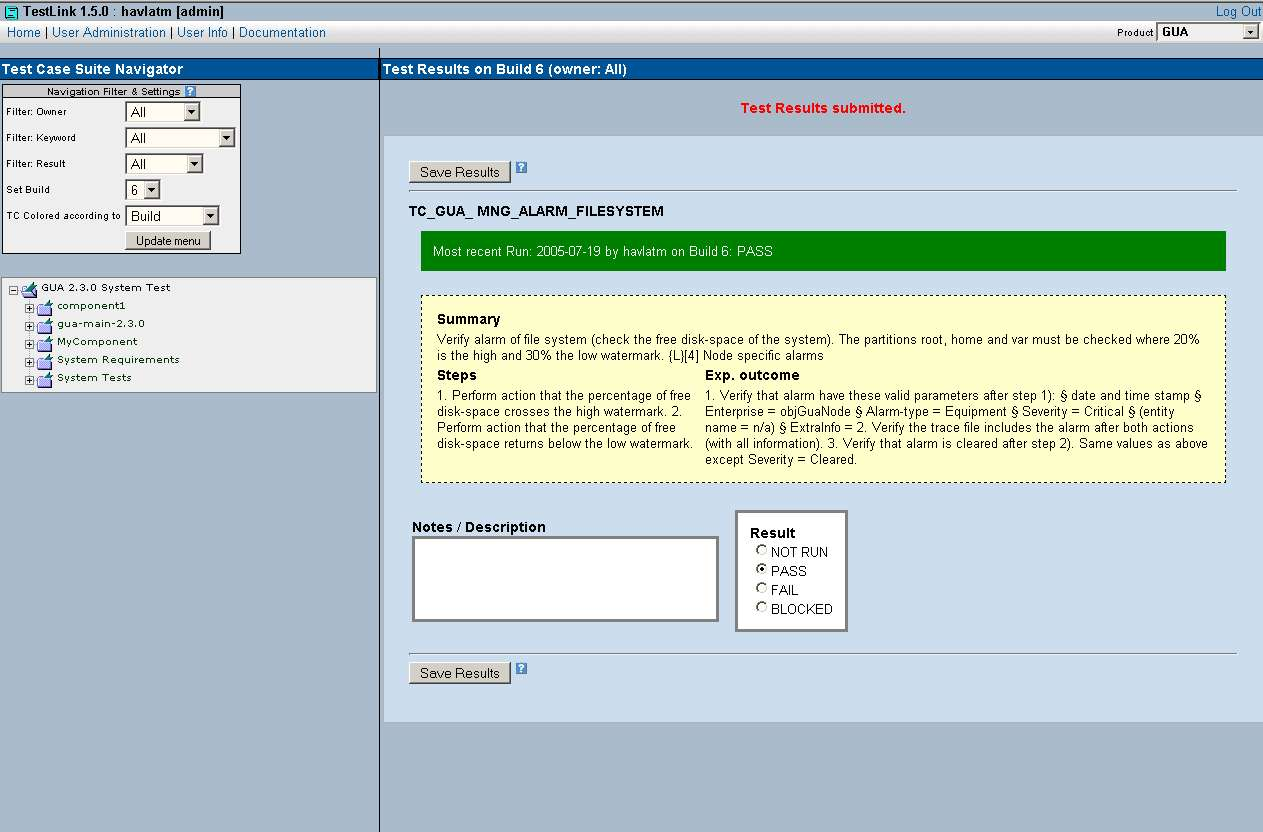
\includegraphics[width=0.8\textwidth]{testlink}
		\end{center}
		\caption{TestLink - acompanhamento/suporte ~\cite{siteTestLink}}
		\label{fig:testlink}
	\end{figure}

As ferramentas de automação de teste visam facilitar o processo de teste e podem auxiliar no desenvolvimento dos testes, execução, manuseio das informações de resultado e a comunicação entre os envolvidos no processo. Utilizando \textit{scripts} essas ferramentas são capazes de simular a utilização da aplicação por um ou vários usuários e, além disso, podem ser simulados vários cenários de uso. As ferramentas de teste podem ser divididas em três grupos: desenvolvimento, execução ~\ref{fig:jmeter} e acompanhamento/suporte ~\ref{fig:testlink}.

	\begin{figure}[!htbp]
		\begin{center}
			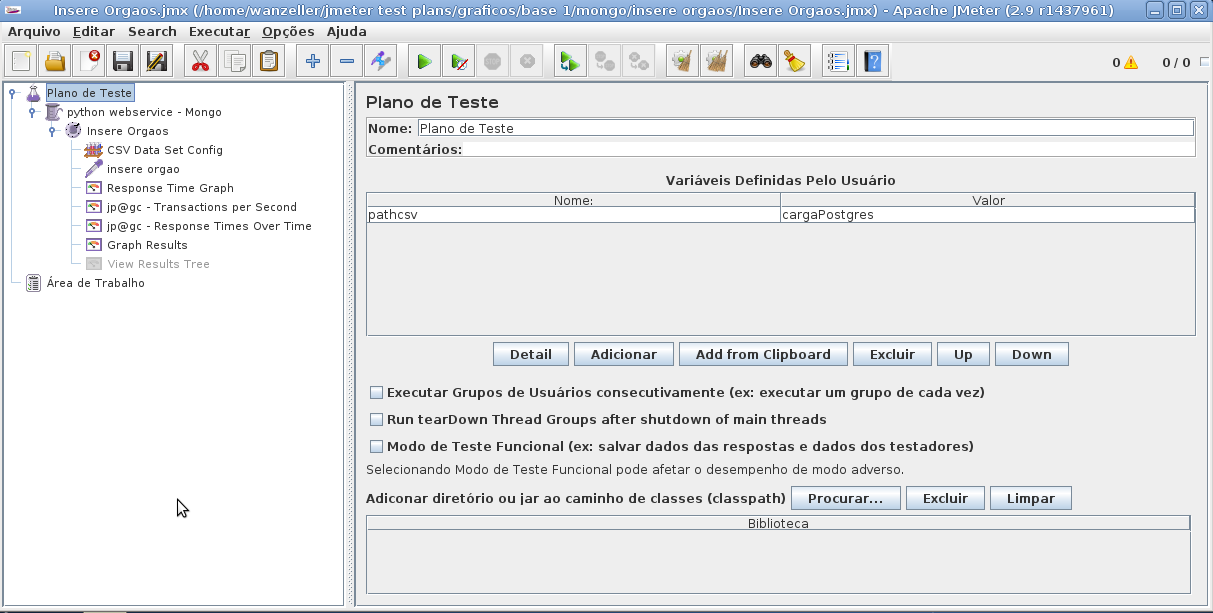
\includegraphics[width=0.8\textwidth]{jmeter}
		\end{center}
		\caption{JMeter - Ferramenta para execução de testes ~\cite{siteJmeter}}
		\label{fig:jmeter}
	\end{figure}


\subsection{JMeter}

O Apache JMeter é uma aplicação \textit{open source}, 100\% desenvolvida em Java e que foi criada para a execução de testes de carca e para medição de performance. Foi originalmente criado para testar aplicações web. O JMeter pode ser usado para testar a performance tanto de recursos estáticos quanto de recursos dinâmicos  (arquivos, servelts, scripts Perl, objetos Java, Bancos de dados e queries, Servidores FTP e etc ). Com ele é possível simular cargas pesadas em um servidor, rede ou objeto para testar o seu comportamento ou para analisar a performance em diferentes tipos de carga ~\cite{siteJmeter}.

O JMeter pode testar diferentes tipos de servidores como:

\begin{itemize}
\item Web - HTTP, HTTPS
\item SOAP
\item Database via JDBC
\item LDAP
\item JMS
\item Mail - SMTP, POP3 e IMAP
\item Comandos nativos ou scripts shell
\end{itemize}

Para realizarmos testes no JMeter precisamos criar um plano de teste. O plano de teste descreve uma série de passos que o JMeter terá de executar. O plano de teste pode conter os seguintes elementos: Grupo de Thread, controladores lógicos, testadores, ouvintes, \textit{timers}, \textit{assertions} e elementos de configuração. A seguir vamos ver os elementos que serão usados nos planos de teste desse trabalho.

Quando iniciamos o nosso plano de teste, o primeiro item que devemos procurar é o testador. Os testadores basicamente enviam requisições aos servidores e aguardam retorno. Cada testador possui diversas configurações que podem ser customizadas.

\begin{description}
\item[ Testador de Requisição SOAP/XML - RPC] \hfill \\

O testador SOAP (figura \ref{fig:testador_insere_orgao}) é usado para mandar requisições SOAP para um Web service.  Ele cria uma requsição HTTP POST com os dados especificados e executa o POST.  As principais configurações são:


\begin{itemize}
\item \textbf{URL}:  Endereço do WSDL do Web service.
\item \textbf{Ação SOAP}: Endereço da requisição SOAP que o testador utilizará.
\item \textbf{Dados SOAP/XML-RPC}: Requisição que será enviada para o Web service. Deve estar em formato XML.
\end{itemize}

	\begin{figure}[!htbp]
		\begin{center}
			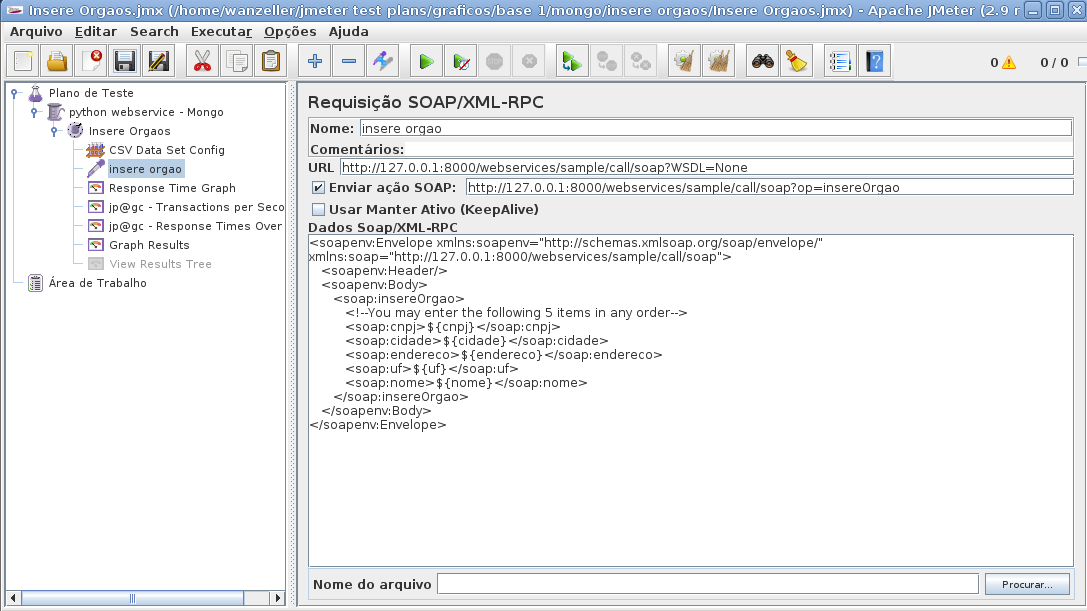
\includegraphics[width=1\textwidth]{testador_insere_orgao}
		\end{center}
		\caption{Testador de Requisição SOAP/XML - RPC}
		\label{fig:testador_insere_orgao}
	\end{figure}
	
\end{description}

Os ouvintes nos permite ter acesso às informações geradas pelo JMeter durante os testes. Temos ouvintes que geram gráficos, gravam informações em arquivos, listam o retorno das requisições e outros vários. A seguir veremos o gráfico de resultados e o gráfico de tempo de resposta.

\begin{description}
\item[Gráfico de Resultados] \hfill \\

O gráfico de resultados gera um gráfico com os tempos de todas as requisições. Na legenda do gráfico temos o tempo da requisição atual (preto), a média atual de todas as requisições (azul), a derivação atual (vermelho), e a vazão atual (verde), todas em milisecundos. A vazão representa o número de transações por minuto (os atrazos causados pelo processamento interno do JMeter não são considerados).

\item[Gráfico de Tempo de Resposta] \hfill \\

O gráfico de tempo de resposta plota uma linha no gráfico que descreve a evolução do tempo de resposta de cada requisição durante o teste.
\end{description}

Os elementos de configuração podem ser utilizadoos para configurar padrões e variáveis que serão utilizadas pelos testadores.

\begin{description}
\item[Elemento para Configuração de Dados CSV] \hfill \\

Esse elemento de configuração é usado para ler linhas de um arquivo e armazená-las em variáveis.Podemos ver um exemplo na figura \ref{fig:configuracao_csv}. Para realizar os testes de inserção de dados no banco esse elemento será de grande importância.

	\begin{figure}[!htbp]
		\begin{center}
			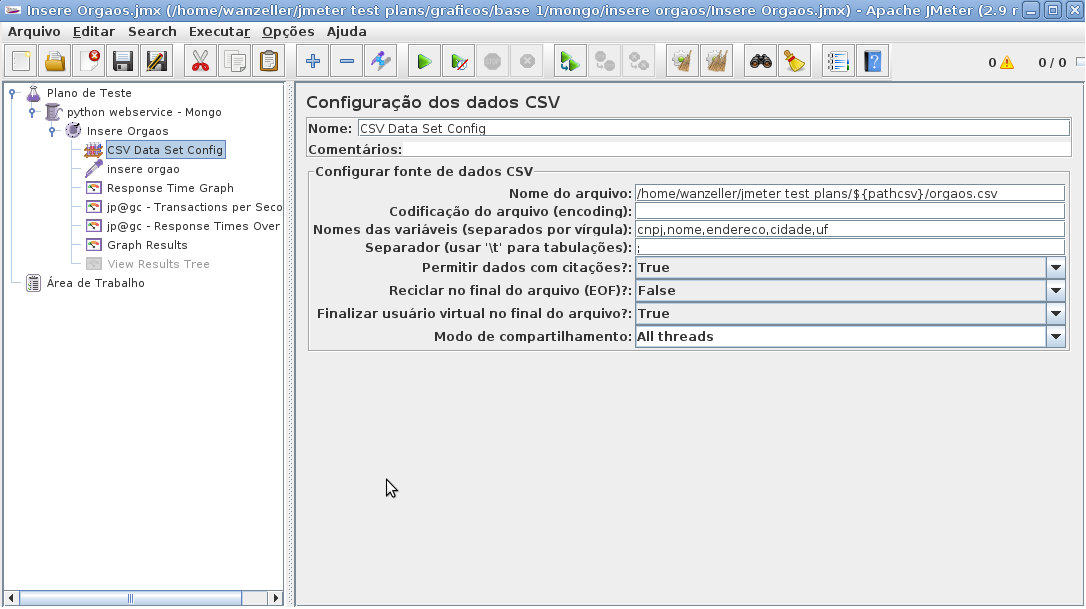
\includegraphics[width=1\textwidth]{configuracao_csv}
		\end{center}
		\caption{Elemento de Configuração de Dados CSV}
		\label{fig:configuracao_csv}
	\end{figure}
	
\end{description}














